\documentclass{article}
\title{\textbf{Laboratorio 04 \\ Tema: Python}}
\author{Melsy Melany Huamaní Vargas}

\usepackage{fancyhdr}
\usepackage{graphicx}
\usepackage{geometry}
\geometry{top=3cm,a4paper,right=2.5cm}
\usepackage{hyperref}

\usepackage[utf8]{inputenc}
\usepackage[T1]{fontenc}
\usepackage[spanish]{babel}
\usepackage{times}

\usepackage{color}
\definecolor{gray97}{gray}{.97}
\definecolor{gray75}{gray}{.75}
\definecolor{gray45}{gray}{.45}

\usepackage{listings}
\lstset{ frame=Ltb,
framerule=0pt,
aboveskip=0.5cm,
framextopmargin=3pt,
framexbottommargin=3pt,
framexleftmargin=0.4cm,
framesep=0pt,
rulesep=.4pt,
backgroundcolor=\color{gray97},
rulesepcolor=\color{black},
%
stringstyle=\ttfamily,
showstringspaces = false,
basicstyle=\small\ttfamily,
commentstyle=\color{gray45},
keywordstyle=\bfseries,
%
numbers=left,
numbersep=15pt,
numberstyle=\tiny,
numberfirstline = false,
breaklines=true,
%
xleftmargin=30pt,
}

\lstnewenvironment{listing}[1][]
{\lstset{#1}\pagebreak[0]}{\pagebreak[0]}

\lstdefinestyle{shell}
{basicstyle=\scriptsize\bf\ttfamily,
backgroundcolor=\color{gray75},
language=sh,
numbers=none,
}

\lstdefinestyle{python}
{language=python,
}

\pagestyle{fancy}
\fancyhf{}
\fancyhead[L]{
\includegraphics[height=1cm]{imagenes/epis.png}}
\fancyhead[C]{\fontsize{7}{8}\selectfont
\begin{tabular}{c}
  UNIVERSIDAD NACIONAL DE SAN AGUSTIN \\
  FACULTAD DE INGENIERÍA DE PRODUCCIÓN Y SERVICIOS \\
  DEPARTAMENTO ACADÉMICO DE INGENIERÍA DE SISTEMAS E INFORMÁTICA \\
  ESCUELA PROFESIONAL DE INGENIERÍA DE SISTEMAS
\end{tabular}}
\fancyhead[R]{
\includegraphics[height=1cm]{imagenes/abet.png}}


\usepackage{xcolor}
\usepackage{colortbl}
\usepackage{array}

\setlength{\headheight}{2cm}
\begin{document}

\begin{titlepage}
  \maketitle 

  \vspace{2cm}
  
  \begin{center}
    \begin{tabular}{|>{\centering\arraybackslash}p{3cm}|>{\centering\arraybackslash}p{3cm}|>{\centering\arraybackslash}p{3cm}|}
      \hline
      \rowcolor{red}
      \textcolor{white}{Profesor} & \textcolor{white}{Escuela} & \textcolor{white}{Asignatura} \\
      \hline
      Carlo Corrales Anibal Sardon & Ingeniería de Sistemas & Programación Web 2 \\
      \hline
    \end{tabular}
  \end{center}

  \vspace{5pt}

  \begin{center}
    \begin{tabular}{|>{\centering\arraybackslash}p{3cm}|>{\centering\arraybackslash}p{3cm}|>{\centering\arraybackslash}p{3cm}|}
      \hline
      \rowcolor{red}
      \textcolor{white}{Laboratorio} & \textcolor{white}{Tema} & \textcolor{white}{Duración} \\
      \hline
      04 & Python & 04 horas \\
      \hline
    \end{tabular}
  \end{center}

  \vspace{5pt}

  \begin{center}
    \begin{tabular}{|>{\centering\arraybackslash}p{3cm}|>{\centering\arraybackslash}p{3cm}|>{\centering\arraybackslash}p{3cm}|}
      \hline
      \rowcolor{red}
      \textcolor{white}{Semestre académico} & \textcolor{white}{Fecha de inicio} & \textcolor{white}{Fecha de entrega} \\
      \hline
      2023 - A & 30/05/2023 & 06/06/2023 \\
      \hline
    \end{tabular}
  \end{center}
\end{titlepage}


\noindent
\section*{\centering SOLUCIÓN Y RESULTADOS}

\vspace{2\baselineskip}

\textbf{ENLACE GITHUB Y GIT}

Este trabajo se está presentando en el Github: \url{https://github.com/mhuamanivar/PW2-HuamaniV-Lab04} y el .git es: \url{https://github.com/mhuamanivar/PW2-HuamaniV-Lab04.git}.

\vspace{2\baselineskip}

\textbf{INSTALACIÓN PARA EL USO DE PYTHON}

Se utiliza el subsistema Ubuntu 22.04.2 LTS a través de WSL (Windows Subsystem for Linux) para usar Python y las herramientas necesarias para su uso en estos ejercicios.

\vspace{2\baselineskip}

\begin{itemize}
  \item Primero se verifica la versión de Python.

  \begin{lstlisting}[style=shell]
  melsy@bonne:~$ python3 --version
  Python 3.10.6
  \end{lstlisting}

  \item Luego actualizamos los paquetes del sistema de Linux.

  \begin{lstlisting}[style=shell]
  melsy@bonne:~$ sudo apt-get update
  [sudo] password for melsy:
  Get:1 http://security.ubuntu.vom.ubuntu jammy-security InRelease [110 kB]
  Hit:2 http://archive.ubuntu.vom.ubuntu jammy InRelease
  Get:3 http://archive.ubuntu.vom.ubuntu jammy-updates InRelease [119 kB]
  Get:4 http://security.ubuntu.vom.ubuntu jammy-security/main amd64 Packages [442 kB]
  ...
  \end{lstlisting}
  
  \item Después se instala pip, una herramienta que (también) instala y administra los paquetes de programación que queramos usar en nuestros proyectos de desarrollo.

  \begin{lstlisting}[style=shell]
  melsy@bonne:~$ sudo apt-get install -y python3-pip
  Reading package lists... Done
  Building dependency tree... Done
  Reading state information... Done
  ...
  \end{lstlisting}
  
  \item Se instalan paquetes y herramientas de desarrollo que garantizan una configuración sólida para nuestro entorno de programación.

  \begin{lstlisting}[style=shell]
  melsy@bonne:~$ sudo apt-get install build-essential libssl-dev libffi-dev python3-dev
  Reading package lists... Done
  Building dependency tree... Done
  Reading state information... Done
  build-essential is already the newest version (12.9ubuntu3).
  ...
  \end{lstlisting}
  
  \item Después, se configura un entorno virtual, los cuales permiten tener un espacio aislado en los proyectos Python y garantizan que puedan tener su propio conjunto de dependencias, como diferentes versiones de los paquetes o varios entornos de programación. En este caso, se usa el módulo venv, que es parte de la biblioteca estándar de Python y se instala de la siguiente forma.

  \begin{lstlisting}[style=shell]
  melsy@bonne:~$ sudo apt install -y python3-venv
  Reading package lists... Done
  Building dependency tree... Done
  Reading state information... Done
  ...
  \end{lstlisting}
  
  \item Luego se crea el directorio en donde queremos crear el entorno virtual y se ingresa con ``cd``.

  \begin{lstlisting}[style=shell]
  melsy@bonne:~$ mkdir -p ~/univ/pw2/lab04/my_env
  melsy@bonne:~$ cd ~/univ/pw2/lab04/my_env
  \end{lstlisting}
  
  \item En el directorio se crea un entorno virtual ejecutando el siguiente comando.

  \begin{lstlisting}[style=shell]
  melsy@bonne:~/univ/pw2/lab04/my_env$ virtualenv -p python3 .
  created virtual environment CPython3.10.6.final.0-64 in 137ms
    creator CPython3Posix(dest=/home/melsy/univ/pw2/lab04/my_env, clear=False, no_vcs_ignore=False, global=False)
    seeder FromAppData(download=False, pip=bundle, setuptools=bundle, wheel=bundle, via=copy, app_data_dir=/home/melsy/.local/share/virtualenv)
      added seed packages: pip==22.0.2, setuptools==59.6.0, wheel==0.37.1
    activators BashActivator,CShellActivator,FishActivator,NushellActivator,PowerShellActivator,PythonActivator
  melsy@bonne:~/univ/pw2/lab04/my_env$ mkdir -p ~/univ/pw2/lab04/my_env/src
  melsy@bonne:~/univ/pw2/lab04/my_env$ cd ~/univ/pw2/lab04/my_env/src
  \end{lstlisting}
  
  \item Ahora se activa el entorno virtual.

  \begin{lstlisting}[style=shell]
  melsy@bonne:~/univ/pw2/lab04/my_env/src$ source ../bin/activate
  (my_env) melsy@bonne:~/univ/pw2/lab04/my_env/src$
  \end{lstlisting}
  
  \item Se crea un archivo ``hello.py`` para probar la ejecución de un archivo Python.

  \begin{lstlisting}[style=shell]
  (my_env) melsy@bonne:~/univ/pw2/lab04/my_env/src$ vim hello.py
  \end{lstlisting}
  
  \item Se edita el archivo 'hello.py', colocando lo siguiente.

  \begin{lstlisting}[style=python]
  print("Hello, World!")
  \end{lstlisting}
  
  \item Se sale de vim con ``Esc``, luego se escribe ``:wq`` para guardar y salir del archivo. Luego se ejecuta el archivo Python.

  \begin{minipage}{\linewidth}
    \centering
    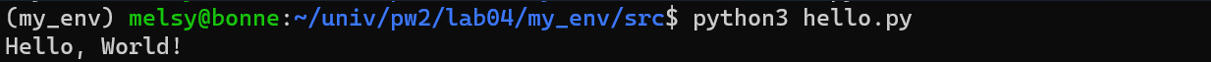
\includegraphics[width=0.9\textwidth]{imagenes/hello.png}
  \end{minipage}

  
  \item Se ve que se ejecutó correctamente. Para desactivar el entorno virtual, se utiliza el siguiente comando.

  \begin{lstlisting}[style=shell]
  (my_env) melsy@bonne:~/univ/pw2/lab04/my_env/src$ deactivate
  melsy@bonne:~/univ/pw2/lab04/my_env/src$
  \end{lstlisting}
\end{itemize}

\pagebreak

\subsection*{I. EJERCICIOS RESUELTOS}

\vspace{\baselineskip}

Se activa el entorno virtual y se crean los directorios donde trabajaremos los ejercicios resueltos.

\begin{lstlisting}[style=shell]
melsy@bonne:~/univ/pw2/lab04/my_env/src$ source ../bin/activate
(my_env) melsy@bonne:~/univ/pw2/lab04/my_env/src$ mkdir resueltos
(my_env) melsy@bonne:~/univ/pw2/lab04/my_env/src$ cd resueltos/
(my_env) melsy@bonne:~/univ/pw2/lab04/my_env/src/resueltos$
\end{lstlisting} 

\vspace{2\baselineskip}

\textbf{1. Determinar si una matriz de tamaño N x N es escalar.}

  \vspace{\baselineskip}

  \begin{itemize}
  \item Se crea el archivo ``esEscalar.py``.
  
  \begin{lstlisting}[style=python]
  def esEscalar(m):
      d = m[0][0]
      for i in range(len(m)):
          for j in range(len(m)):
              if i != j:
                  if m[i][j] != 0:
                      print(m[i][j])
                      return False
              elif m[i][j] != d:
                  print(m[i][j])
                  return False
      return True
  \end{lstlisting}
  
  \item Se crea el archivo ``test\_esEscalar.py``, en el cual importamos el archivo anterior como función.
  
  \begin{lstlisting}[style=python]
  import esEscalar as fu

  def prueba(M):
      if fu.esEscalar(M):
          print("Si es escalar")
      else:
          print("No es escalar")

  #Z = [[1, 2, 3], [4, 5, 6], [7, 8, 9]]
  #Z = [[1, 2, 3], [4, 1, 6], [7, 8, 1]]
  Z = [[1, 0, 0], [0, 1, 0], [0, 0, 1]]

  prueba(Z)
  \end{lstlisting}

  \item Se ejecuta el archivo ``test\_esEscalar.py`` con la matriz de prueba que no está comentada.
  
  \begin{minipage}{\linewidth}
    \centering
    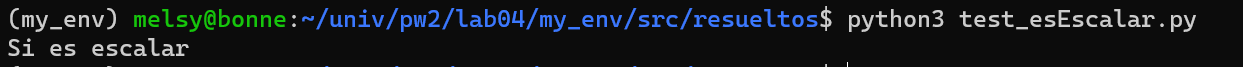
\includegraphics[width=0.9\textwidth]{imagenes/r_escalar.png}
  \end{minipage}

  \end{itemize}
    
  \pagebreak

\textbf{2. Determinar si una matriz de tamaño N x N es unitaria.}
  
  \vspace{\baselineskip}

  \begin{itemize}
  
  \item Se crea el archivo ``esUnitaria.py``.

  \begin{lstlisting}[style=python]
  import esEscalar as fu

  def esUnitaria(m):
      return m[0][0] == 1 and fu.esEscalar(m)
  \end{lstlisting}

    
  \item Se crea el archivo ``test\_esUnitaria.py``, en el cual importamos el archivo anterior como función.
    
  \begin{lstlisting}[style=python]
  import esUnitaria as fu

  def prueba(M):
      if fu.esUnitaria(M):
          print("Si es unitaria")
      else:
          print("No es unitaria")

  #Z = [[1, 2, 3], [4, 5, 6], [7, 8, 9]]
  #Z = [[1, 2, 3], [4, 1, 6], [7, 8, 1]]
  Z = [[2, 0, 0], [0, 2, 0], [0, 0, 2]]
  #Z = [[1, 0, 0], [0, 1, 0], [0, 0, 1]]

  prueba(Z)
  \end{lstlisting}

  \item Se ejecuta el archivo ``test\_esUnitaria.py`` con la matriz de prueba que no está comentada.

  \begin{minipage}{\linewidth}
    \centering
    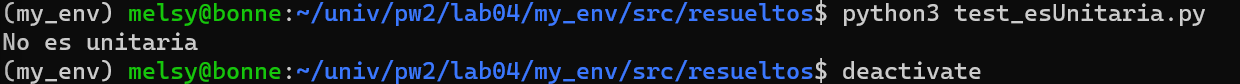
\includegraphics[width=0.9\textwidth]{imagenes/r_unitaria.png}
  \end{minipage}

  \end{itemize}

\pagebreak

\subsection*{II. EJERCICIOS PROPUESTOS}

  \vspace{\baselineskip}

  En este caso como se estaba trabajando en WSL, no está permitido el uso de gráficos como ``pygame``, por lo que se trabajó en el sistema principal Windows. Por lo que se crea un nuevo ambiente y lo activamos.
  
  \begin{lstlisting}[style=shell]
  C:\Users\melsy\Lab04>python -m venv my_env
  C:\Users\melsy\Lab04>my_env\Scripts\activate
  \end{lstlisting}
  
  \vspace{\baselineskip}

  Ahora se actualiza el pip de python en Windows.

  \begin{lstlisting}[style=shell]
  (my_env) C:\Users\melsy\Lab04>python.exe -m pip install --upgrade pip
  Requirement already satisfied: pip in c:\users\melsy\lab04\my_env\lib\site-packages (22.3.1)
  Collecting pip
    Downloading pip-23.1.2-py3-none-any.whl (2.1 MB)
      -------------------------------- 2.1/2.1 MB 848.2 kB/s eta 0:00:00
  Installing collected packages: pip
    Attempting uninstall: pip
      Found existing installation: pip 22.3.1
      Uninstalling pip-22.3.1:
        Successfully uninstalled pip-22.3.1
  Successfully installed pip-23.1.2
  \end{lstlisting}

  \vspace{\baselineskip}

  Posteriormente se instala pygame para mostrar los gráficos.
  
  \begin{lstlisting}[style=shell]
  (my_env) C:\Users\melsy\Lab04>pip3 install pygame
  Collecting pygame
    Downloading pygame-2.4.0-cp311-cp311-win_amd64.whl (10.6 MB)
      -------------------------------- 10.6/10.6 MB 531.0 kB/s eta 0:00:00
  Installing collected packages: pygame
  Successfully installed pygame-2.4.0
  \end{lstlisting}

  \vspace{\baselineskip}

  Luego se ingresa a una carpeta ya creada llamada ``propuestos``, donde (como dice el nombre) se guardarán todos los ejercicios propuestos.
  
  \begin{lstlisting}[style=shell]
  (my_env) C:\Users\melsy\Lab04>cd my_env\Scripts\propuestos
  (my_env) C:\Users\melsy\Lab04\my_env\Scripts\propuestos>
  \end{lstlisting}

  \vspace{2\baselineskip}

  \textbf{1. Implementar los métodos de la clase Picture.}

  \vspace{\baselineskip}

  Una vez guardados los archivos dados por el profesor se deben realizar pruebas para realizar los métodos que son dados en este primer ejercicio propuesto.
  
  \begin{lstlisting}[style=shell]
  (my_env) C:\Users\melsy\Lab04\my_env\Scripts\propuestos>python
  Python 3.11.1 (tags/v3.11.1:a7a450f, Dec  6 2022, 19:58:39) [MSC v.1934 64 bit (AMD64)] on win32
  Type "help", "copyright", "credits" or "license" for more information.
  >>> from chessPictures import *
  >>> from interpreter import draw
  pygame 2.4.0 (SDL 2.26.4, Python 3.11.1)
  Hello from the pygame community. https://www.pygame.org/contribute.html
  \end{lstlisting}

  \pagebreak

  Ahora se realizan los métodos a continuación:

  \vspace{\baselineskip}

  \begin{itemize}

  \item \textbf{verticalMirror:} Devuelve el espejo vertical de la imagen
  
  \vspace{\baselineskip}

  Se crea un arreglo vacío ``vertical`` en donde se coloca poco a poco cada valor del arreglo de la imagen dada, de manera que cada string parte de ese arreglo se invierta utilizando ``[::-1]``, de esta manera como cada elemento se está inviertando se obtiene un resultado en forma de reflejo vertical de la imagen.
  
    \begin{lstlisting}[style=python]
    def verticalMirror(self):
        vertical = []
        for value in self.img:
            vertical.append(value[::-1])
        return Picture(vertical)
    \end{lstlisting}

    \vspace{\baselineskip}

    \begin{itemize}
      \item Para probar utilizamos el siguiente comando

      \begin{lstlisting}[style=shell]
      >>> draw(knight)
      \end{lstlisting}
      \begin{minipage}{\linewidth}
        \centering
        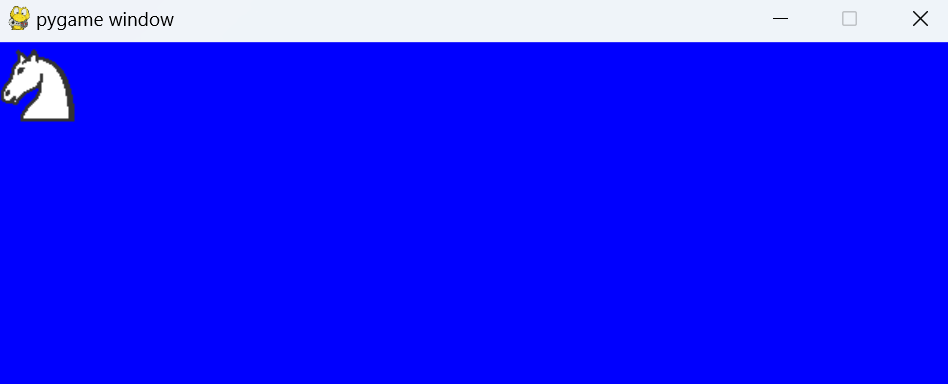
\includegraphics[width=0.9\textwidth]{imagenes/p_vertical1.png}
      \end{minipage}

      \vspace{2\baselineskip}

      \item Luego comparamos al utilizar el siguiente comando, para ver que funcionó correctamente
      \begin{lstlisting}[style=shell]
      >>> draw(knight.verticalMirror())
      \end{lstlisting}
      \begin{minipage}{\linewidth}
        \centering
        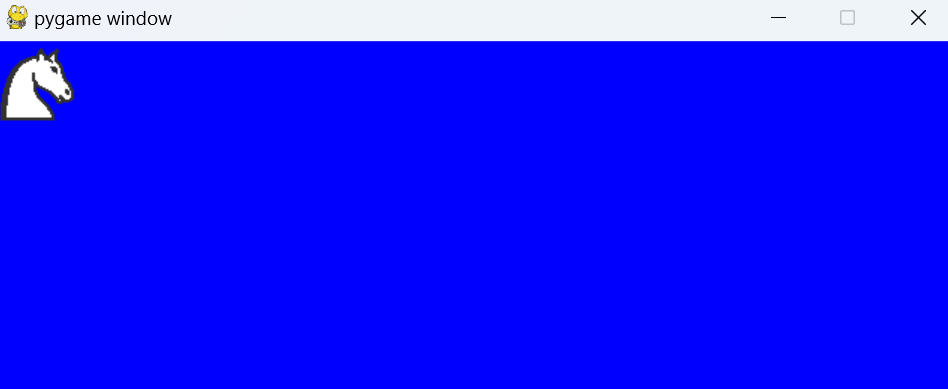
\includegraphics[width=0.9\textwidth]{imagenes/p_vertical2.png}
      \end{minipage}
    \end{itemize}

  \pagebreak

  \item \textbf{horizontalMirror:} Devuelve el espejo horizontal de la imagen
  
  \vspace{\baselineskip}

  Se crea un arreglo vacío ``horizontal`` en el cual se almacena el arreglo invertido del atributo ``img`` del picture, se esta manera se obtiene un espejo horizontal de la figura, de la misma forma que el anterior para invertir el arreglo se utiliza ``[::-1]``.  

    \begin{lstlisting}[style=python]
    def horizontalMirror(self):
          horizontal = self.img[::-1]
          return Picture(horizontal)
    \end{lstlisting}

    \vspace{\baselineskip}

    \begin{itemize}
      \item Para probar utilizamos el siguiente comando

      \begin{lstlisting}[style=shell]
      >>> draw(rock)
      \end{lstlisting}
      \begin{minipage}{\linewidth}
        \centering
        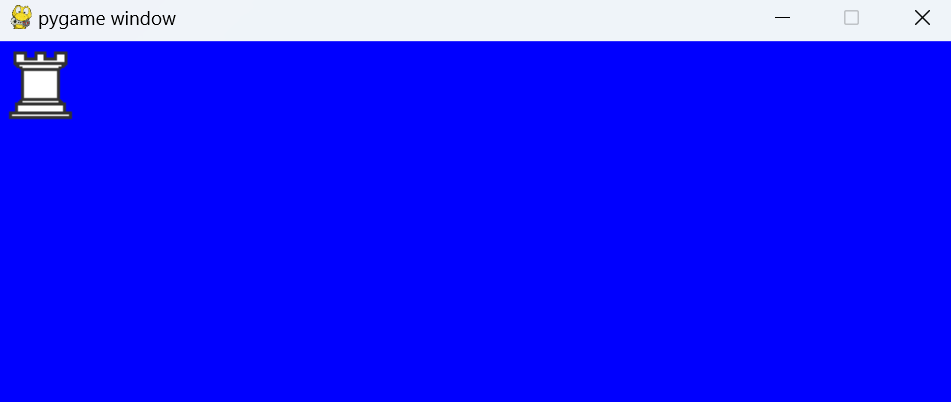
\includegraphics[width=0.9\textwidth]{imagenes/p_horizontal1.png}
      \end{minipage}

      \vspace{2\baselineskip}

      \item Luego comparamos al utilizar el siguiente comando, para ver que funcionó correctamente
      \begin{lstlisting}[style=shell]
      >>> draw(rock.horizontalMirror())
      \end{lstlisting}
      \begin{minipage}{\linewidth}
        \centering
        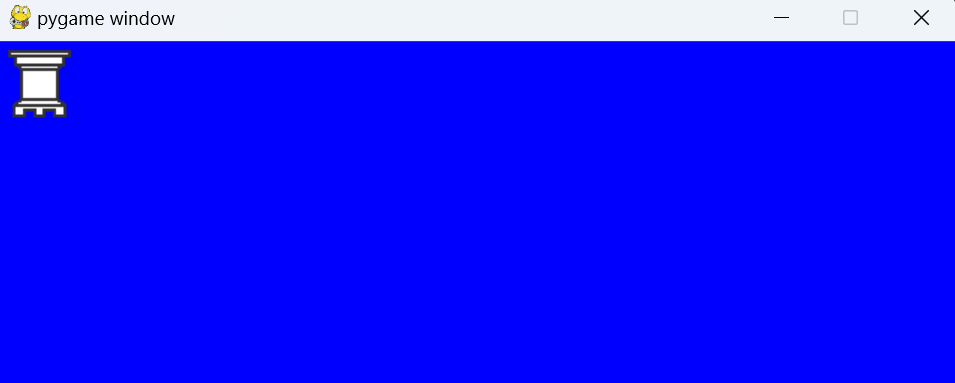
\includegraphics[width=0.9\textwidth]{imagenes/p_horizontal2.png}
      \end{minipage}
    \end{itemize}

  \pagebreak  

  \item \textbf{negative:} Devuelve un negativo de la imagen
  
  \vspace{\baselineskip}

  Se crea un nuevo arreglo ``negative``, el cual por cada valor del arreglo del atributo ``img`` del picture, se invertira los colores al utilizar el método ``\_invColor()``, luego se unen utilizando el método ``join()`` a un solo string y se devuelve como un nuevo elemento del nuevo arreglo creado.  
    
    \begin{lstlisting}[style=python]
    def negative(self):
        negative = []
        for value in self.img:
            invertedColor = "".join([self._invColor(c) for c in value])
            negative.append(invertedColor)
        return Picture(negative)
    \end{lstlisting}

    \vspace{\baselineskip}

    \begin{itemize}
      \item Para probar utilizamos el siguiente comando

      \begin{lstlisting}[style=shell]
      >>> draw(queen)
      \end{lstlisting}
      \begin{minipage}{\linewidth}
        \centering
        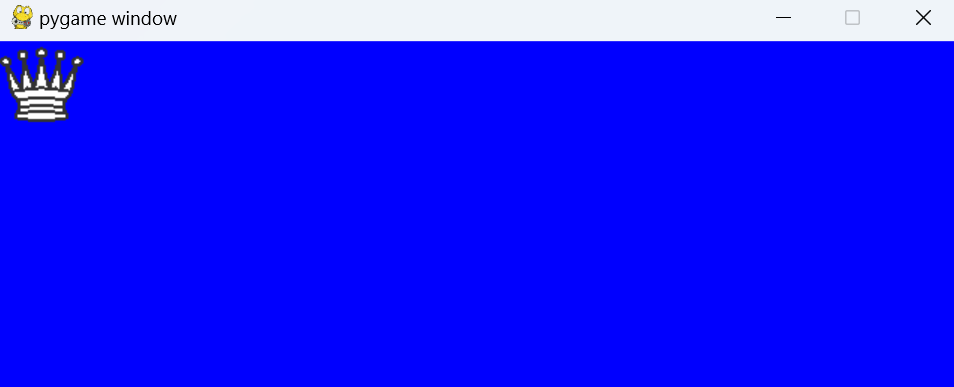
\includegraphics[width=0.9\textwidth]{imagenes/p_negative1.png}
      \end{minipage}

      \vspace{2\baselineskip}

      \item Luego comparamos al utilizar el siguiente comando, para ver que funcionó correctamente
      \begin{lstlisting}[style=shell]
      >>> draw(queen.negative())
      \end{lstlisting}
      \begin{minipage}{\linewidth}
        \centering
        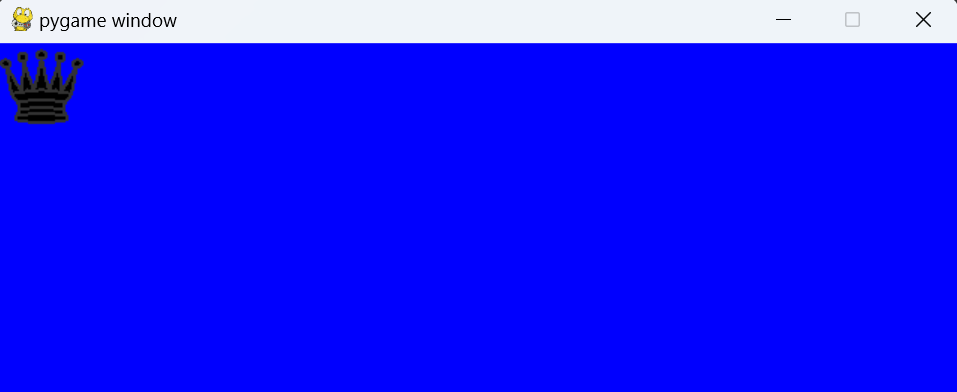
\includegraphics[width=0.9\textwidth]{imagenes/p_negative2.png}
      \end{minipage}
    \end{itemize}

  \pagebreak

  \item \textbf{join:} Devuelve una nueva figura poniendo la figura del argumento al lado derecho de la figura actual
  
  \vspace{\baselineskip}

  Se crea un nuevo arreglo ``joined`` el cual for cada elemento del arreglo del atributo ``img`` del picture actual se agrega el elemento con el mismo índice del arreglo del atributo ``img`` del picture ``p``, de esta manera forman un nuevo arreglo que será almacenado en ``joined``.  

    \begin{lstlisting}[style=python]
    def join(self, p):
        joined = []
        for i in range(len(self.img)):
            joined.append(self.img[i]+p.img[i])
        return Picture(joined)
    \end{lstlisting}

    \vspace{\baselineskip}

    \begin{itemize}
      \item Para probar utilizamos el siguiente comando

      \begin{lstlisting}[style=shell]
      >>> draw(king)
      \end{lstlisting}
      \begin{minipage}{\linewidth}
        \centering
        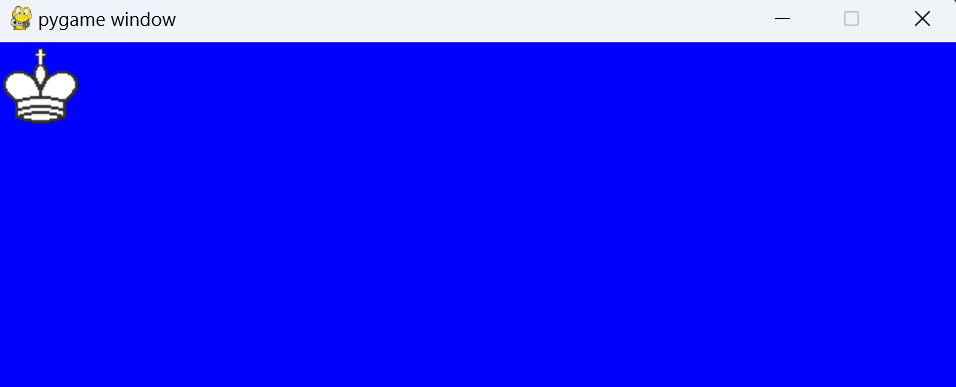
\includegraphics[width=0.9\textwidth]{imagenes/p_join1.png}
      \end{minipage}

      \vspace{2\baselineskip}

      \item Luego comparamos al utilizar el siguiente comando, para ver que funcionó correctamente
      \begin{lstlisting}[style=shell]
      >>> draw(king.join(queen))
      \end{lstlisting}
      \begin{minipage}{\linewidth}
        \centering
        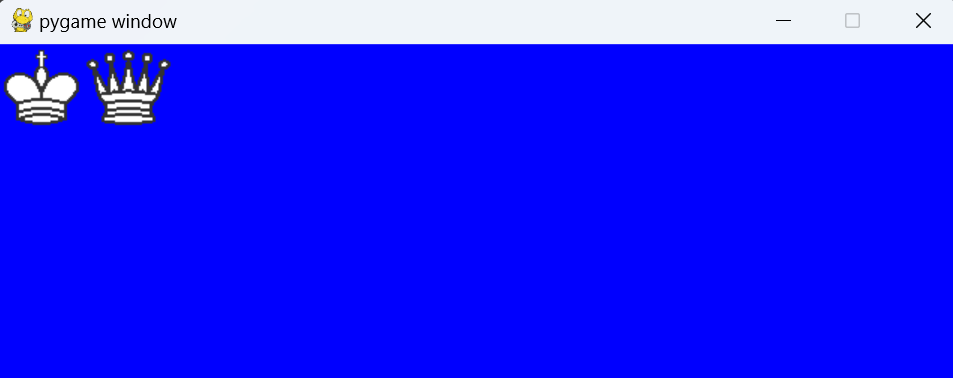
\includegraphics[width=0.9\textwidth]{imagenes/p_join2.png}
      \end{minipage}
    \end{itemize}

  \pagebreak

  \item \textbf{up:} Devuelve una nueva figura poniendo la figura recibida como argumento, encima de la figura actual
  
  \vspace{\baselineskip}

  Se crea un nuevo arreglo ``newFigure`` que almacena el arreglo del atributo ``img`` del picture que es recibido como argumento ``p``, luego se le va añadiendo cada elemento del arreglo ``img`` del picture actual, para que en ``newFigure``, el picture ``p`` se muestre encima del picture actual.  
    \begin{lstlisting}[style=python]
    def up(self, p):
        newFigure = p.img[:]
        for value in self.img:
            newFigure.append(value)
        return Picture(newFigure)
    \end{lstlisting}

    \vspace{\baselineskip}

    \begin{itemize}
      \item Para probar utilizamos el siguiente comando

      \begin{lstlisting}[style=shell]
      >>> draw(bishop)
      \end{lstlisting}
      \begin{minipage}{\linewidth}
        \centering
        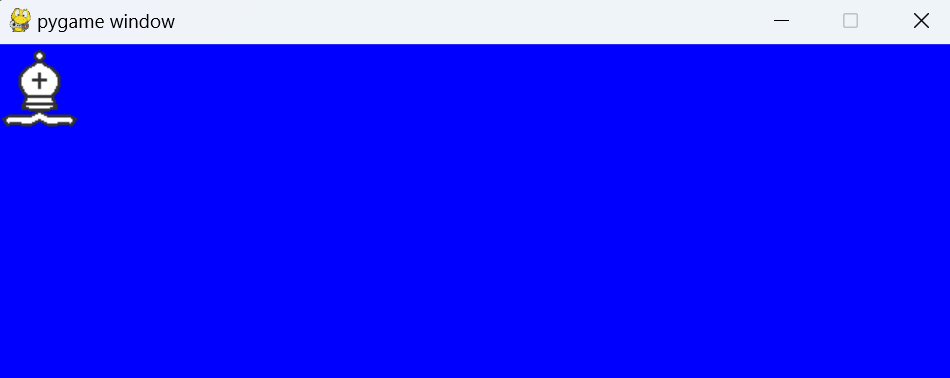
\includegraphics[width=0.9\textwidth]{imagenes/p_up1.png}
      \end{minipage}

      \vspace{2\baselineskip}

      \item Luego comparamos al utilizar el siguiente comando, para ver que funcionó correctamente
      \begin{lstlisting}[style=shell]
      >>> draw(bishop.up(pawn))
      \end{lstlisting}
      \begin{minipage}{\linewidth}
        \centering
        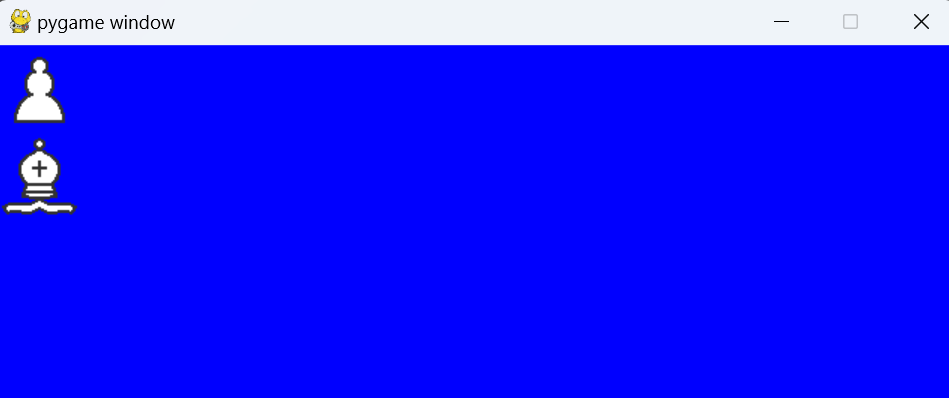
\includegraphics[width=0.9\textwidth]{imagenes/p_up2.png}
      \end{minipage}
    \end{itemize}

  \pagebreak

  \item \textbf{under:} Devuelve una nueva figura poniendo la figura recibida como argumento, sobre la figura actual
  
  \vspace{\baselineskip}

  Se crean las variables ``filas`` y ``columnas`` que almacena el valor adecuado al usar ``range()`` en el arreglo. Luego se crea ``newFigure``, el cual recorrerá por las filas y columnas, de esta forma cuando un caracter del picture actual sea diferente al del picture ``p``, y este último no sea vacío, entonces se priorizará el caracter del picture ``p``, de lo contrario, será del picture actual.

    \begin{lstlisting}[style=python]
    def under(self, p):
        filas = range(len(self.img))
        columnas = range(len(self.img[0]))

        newFigure = []
        for i in filas:
            string = ""
            for j in columnas:
                if (self.img[i][j] != p.img[i][j] and p.img[i][j] != " "):
                    string += p.img[i][j]
                else:
                    string += self.img[i][j]
            newFigure.append(string)
        return Picture(newFigure)
    \end{lstlisting}

    \vspace{\baselineskip}

    \begin{itemize}
      \item Para probar utilizamos el siguiente comando

      \begin{lstlisting}[style=shell]
      >>> draw(square)
      \end{lstlisting}
      \begin{minipage}{\linewidth}
        \centering
        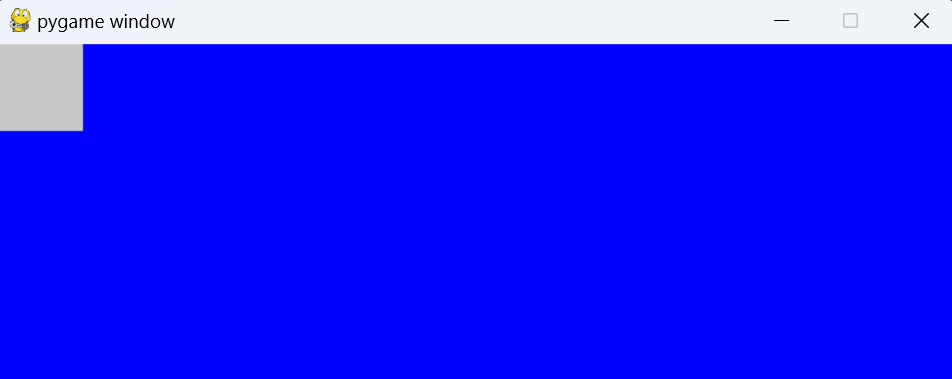
\includegraphics[width=0.9\textwidth]{imagenes/p_under1.png}
      \end{minipage}

      \vspace{2\baselineskip}

      \item Luego comparamos al utilizar el siguiente comando, para ver que funcionó correctamente
      
      \begin{lstlisting}[style=shell]
      >>> draw(square.under(knight))
      \end{lstlisting}

      \begin{minipage}{\linewidth}
        \centering
        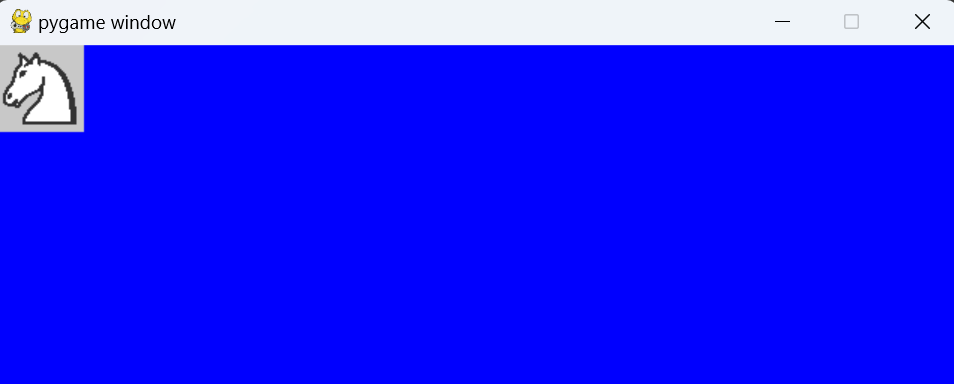
\includegraphics[width=0.9\textwidth]{imagenes/p_under2.png}
      \end{minipage}
    \end{itemize}

  \pagebreak

  \item \textbf{horizontalRepeat::} Devuelve una nueva figura repitiendo la figura actual al costado la cantidad de veces que indique el valor de ``n``
  
  \vspace{\baselineskip}

  Se crea un nuevo arreglo, el cual va almacenando los elementos del arreglo del atributo ``img`` del pciture, y los va multiplicando la cantidad ``n`` introducida, de tal manera que al final se vea de manera repetida horizontalmente la misma figura.  
    
    \begin{lstlisting}[style=python]
    def horizontalRepeat(self, n):
        newFigure = []
        for value in self.img:
            newFigure.append(value*n)
        return Picture(newFigure)
    \end{lstlisting}

    \vspace{\baselineskip}

    \begin{itemize}
      \item Para probar utilizamos el siguiente comando

      \begin{lstlisting}[style=shell]
      >>> draw(rock)
      \end{lstlisting}
      \begin{minipage}{\linewidth}
        \centering
        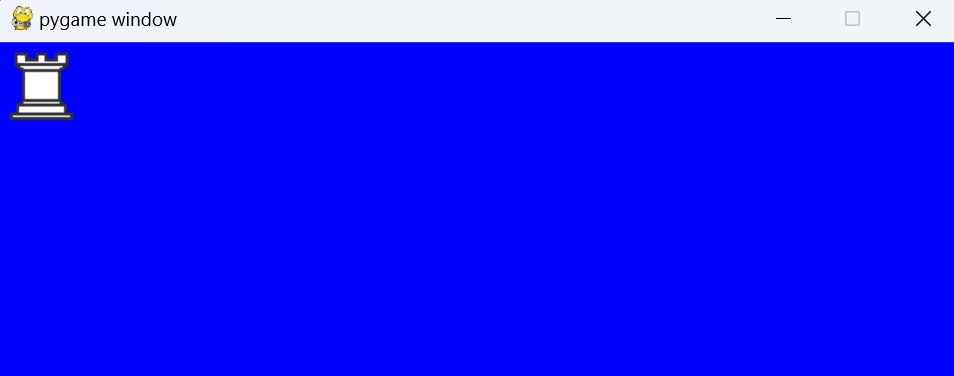
\includegraphics[width=0.9\textwidth]{imagenes/p_horizontalr1.png}
      \end{minipage}

      \vspace{2\baselineskip}

      \item Luego comparamos al utilizar el siguiente comando, para ver que funcionó correctamente
      \begin{lstlisting}[style=shell]
      >>> draw(rock.horizontalRepeat(5))
      \end{lstlisting}
      \begin{minipage}{\linewidth}
        \centering
        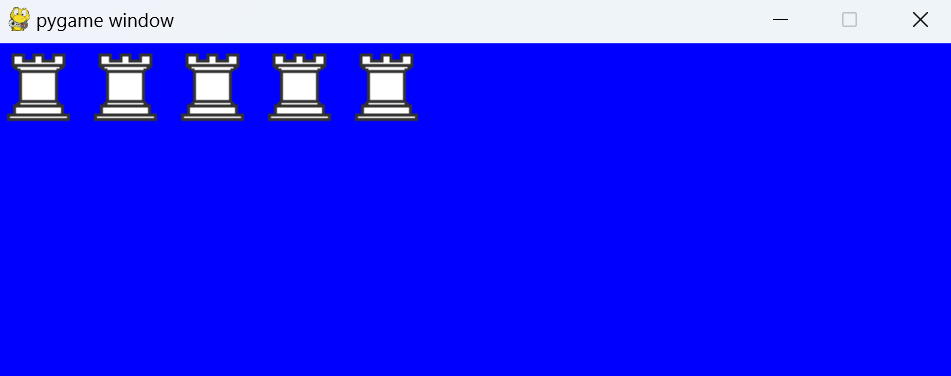
\includegraphics[width=0.9\textwidth]{imagenes/p_horizontalr2.png}
      \end{minipage}
    \end{itemize}

  \pagebreak

  \item \textbf{verticalRepeat:} Devuelve una nueva figura repitiendo la figura actual debajo, la cantidad de veces que indique el valor de ``n``
  
  \vspace{\baselineskip}

  Se crea un nuevo arreglo donde multiplica todo el arreglo del atributo ``img`` del picture, es por ello que en el resultado se ve de manera repetida verticalmente.

    \begin{lstlisting}[style=python]
    def verticalRepeat(self, n):
        newFigure = self.img[:] * n
        return Picture(newFigure)
    \end{lstlisting}

    \vspace{\baselineskip}

    \begin{itemize}
      \item Para probar utilizamos el siguiente comando

      \begin{lstlisting}[style=shell]
      >>> draw(king)
      \end{lstlisting}
      \begin{minipage}{\linewidth}
        \centering
        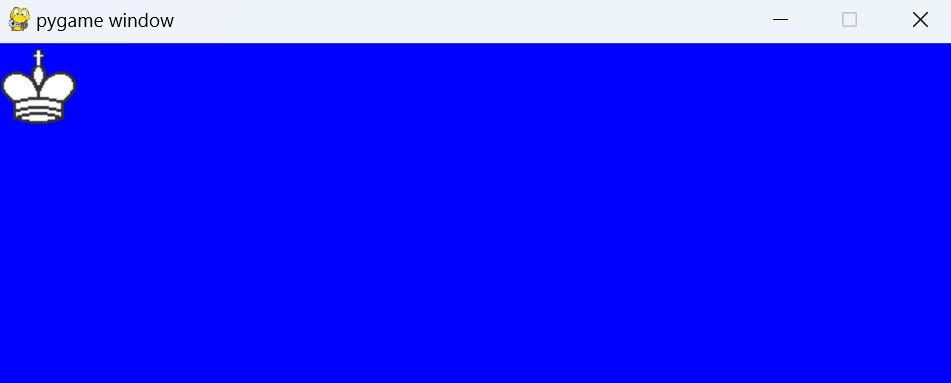
\includegraphics[width=0.9\textwidth]{imagenes/p_verticalr1.png}
      \end{minipage}

      \vspace{2\baselineskip}

      \item Luego comparamos al utilizar el siguiente comando, para ver que funcionó correctamente
      \begin{lstlisting}[style=shell]
      >>> draw(king.verticalRepeat(2))
      \end{lstlisting}
      \begin{minipage}{\linewidth}
        \centering
        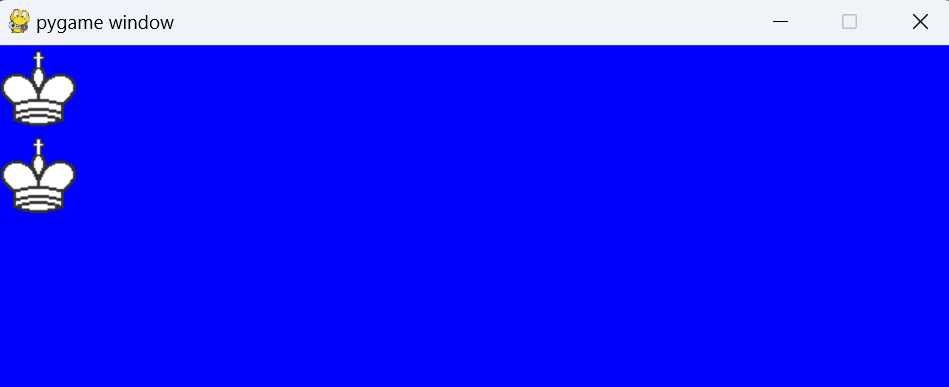
\includegraphics[width=0.9\textwidth]{imagenes/p_verticalr2.png}
      \end{minipage}
    \end{itemize}

  \pagebreak

  \item \textbf{rotate (Extra):} DDevuelve una figura rotada en 90 grados

  \vspace{\baselineskip}

  De la misma forma que en la función ``under()`` se obtienen las filas y columnas. Luego se crea un nuevo arreglo "newFigure", en el cual se irá almacenando el valor correspondiente de las columnas, pero para que vaya rotando entonces colocamos el índice de las filas de manera ``-i``, para obtener el orden inverso solamente de la fila.

    \begin{lstlisting}[style=python]
    def rotate(self):
        """Devuelve una figura rotada en 90 grados """
        filas = range(len(self.img))
        columnas = range(len(self.img[0]))

        newFigure = []
        for i in filas:
            string = ""
            for j in columnas:
                string += self.img[j][-i]
            newFigure.append(string)
        return Picture(newFigure)
    \end{lstlisting}

    \vspace{\baselineskip}

    \begin{itemize}
      \item Para probar utilizamos el siguiente comando

      \begin{lstlisting}[style=shell]
      >>> draw(knight)
      \end{lstlisting}
      \begin{minipage}{\linewidth}
        \centering
        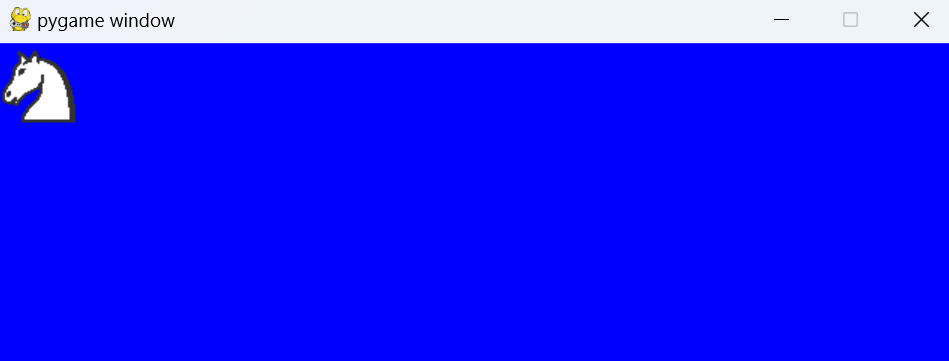
\includegraphics[width=0.9\textwidth]{imagenes/p_rotate1.png}
      \end{minipage}

      \vspace{2\baselineskip}

      \item Luego comparamos al utilizar el siguiente comando, para ver que funcionó correctamente
      \begin{lstlisting}[style=shell]
      >>> draw(knight.rotate())
      \end{lstlisting}
      \begin{minipage}{\linewidth}
        \centering
        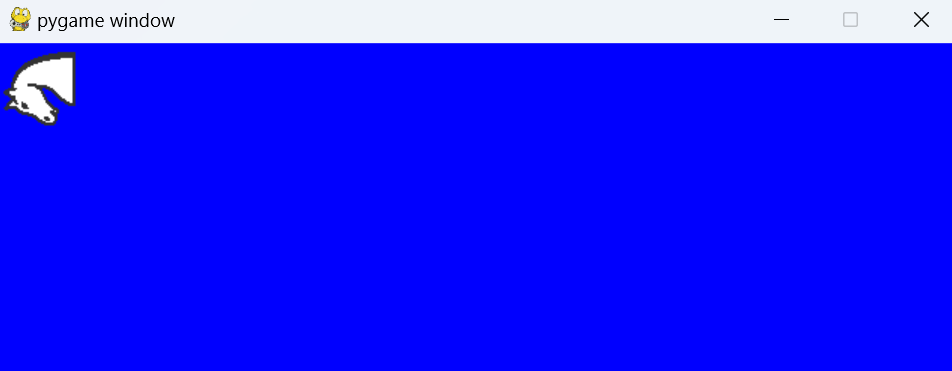
\includegraphics[width=0.9\textwidth]{imagenes/p_rotate2.png}
      \end{minipage}
    \end{itemize}
  
  \end{itemize}

  \pagebreak
  
  \textbf{2. Usando únicamente los métodos de los objetos de la clase Picture dibujar las siguientes figuras.}

  \vspace{\baselineskip}

  Se sale de ``python`` con ``exit()``, pero continuamos en el entorno virtual para probar los ejercicios y demostrar que cumplen de acuerdo a las imágenes pedidas.

  \vspace{\baselineskip}

  \begin{itemize}
  \item \textbf{Se crea el archivo ``Ejercicio2a.py``}
  
  \vspace{\baselineskip}
  
  Utilizando las funciones creadas anteriormente, se contruye de acuerdo a la imagen dada en el laboratorio.

    \begin{lstlisting}[style=python]
    from interpreter import draw
    from chessPictures import *

    wKnight = knight
    bKnight = knight.negative()

    firstKnights = wKnight.join(bKnight)
    secondKnights = bKnight.join(wKnight)

    draw(secondKnights.up(firstKnights))
    \end{lstlisting}

    \vspace{\baselineskip}

    \begin{itemize}
      \item Se ejecuta de la siguiente manera.

      \begin{lstlisting}[style=shell]
      (my_env) C:\Users\melsy\Lab04\my_env\Scripts\propuestos>python Ejercicio2a.py
      pygame 2.4.0 (SDL 2.26.4, Python 3.11.1)
      Hello from the pygame community. https://www.pygame.org/contribute.html
      \end{lstlisting}

      \vspace{2\baselineskip}

      \item El resultado es:
      
      \vspace{\baselineskip}

      \begin{minipage}{\linewidth}
        \centering
        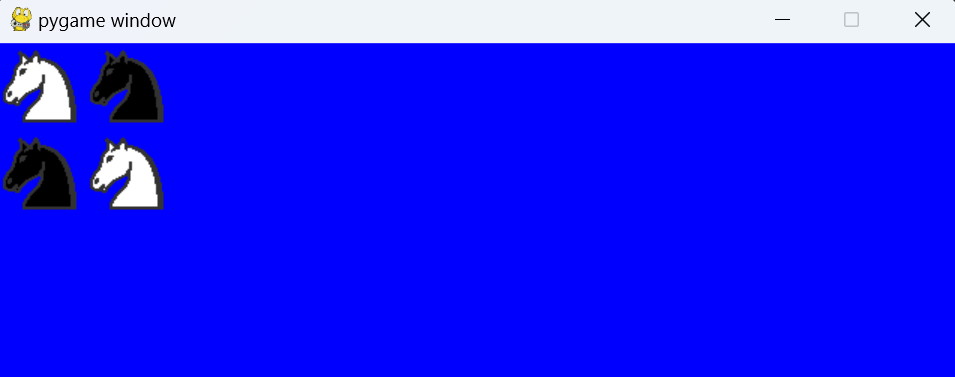
\includegraphics[width=0.9\textwidth]{imagenes/p_ej2a.png}
      \end{minipage}
    \end{itemize}
  
  \pagebreak

  \item \textbf{Se crea el archivo ``Ejercicio2b.py``}
  
  Utilizando las funciones creadas anteriormente, se contruye de acuerdo a la imagen dada en el laboratorio.

  \vspace{\baselineskip}

    \begin{lstlisting}[style=python]
    from interpreter import draw
    from chessPictures import *

    wKnight = knight
    bKnight = knight.negative()

    firstKnights = wKnight.join(bKnight)
    secondKnights = firstKnights.verticalMirror()

    draw(secondKnights.up(firstKnights))
    \end{lstlisting}

    \vspace{\baselineskip}

    \begin{itemize}
      \item Se ejecuta de la siguiente manera.

      \begin{lstlisting}[style=shell]
      (my_env) C:\Users\melsy\Lab04\my_env\Scripts\propuestos>python Ejercicio2b.py
      pygame 2.4.0 (SDL 2.26.4, Python 3.11.1)
      Hello from the pygame community. https://www.pygame.org/contribute.html
      \end{lstlisting}

      \vspace{2\baselineskip}

      \item El resultado es:
      
      \vspace{\baselineskip}

      \begin{minipage}{\linewidth}
        \centering
        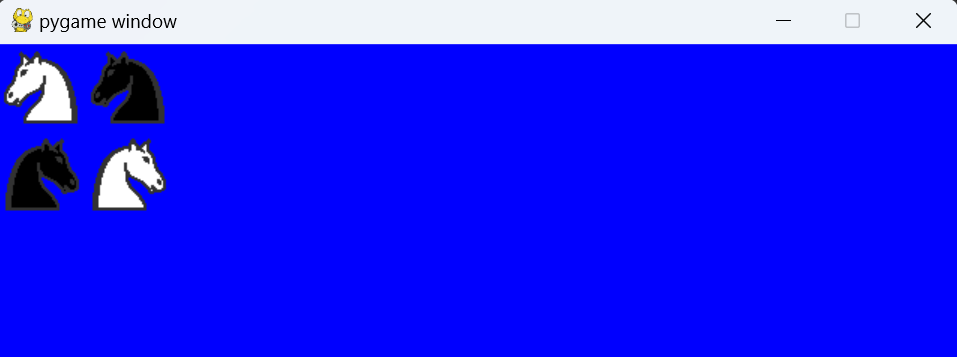
\includegraphics[width=0.9\textwidth]{imagenes/p_ej2b.png}
      \end{minipage}
    \end{itemize}

  \pagebreak

  \item \textbf{Se crea el archivo ``Ejercicio2c.py``}
  
  \vspace{\baselineskip}

  Utilizando las funciones creadas anteriormente, se contruye de acuerdo a la imagen dada en el laboratorio.

    \begin{lstlisting}[style=python]
    from interpreter import draw
    from chessPictures import *

    draw(queen.horizontalRepeat(4))
    \end{lstlisting}

    \vspace{\baselineskip}

    \begin{itemize}
      \item Se ejecuta de la siguiente manera.

      \begin{lstlisting}[style=shell]
      (my_env) C:\Users\melsy\Lab04\my_env\Scripts\propuestos>python Ejercicio2c.py
      pygame 2.4.0 (SDL 2.26.4, Python 3.11.1)
      Hello from the pygame community. https://www.pygame.org/contribute.html
      \end{lstlisting}

      \vspace{2\baselineskip}

      \item El resultado es:
      
      \vspace{\baselineskip}

      \begin{minipage}{\linewidth}
        \centering
        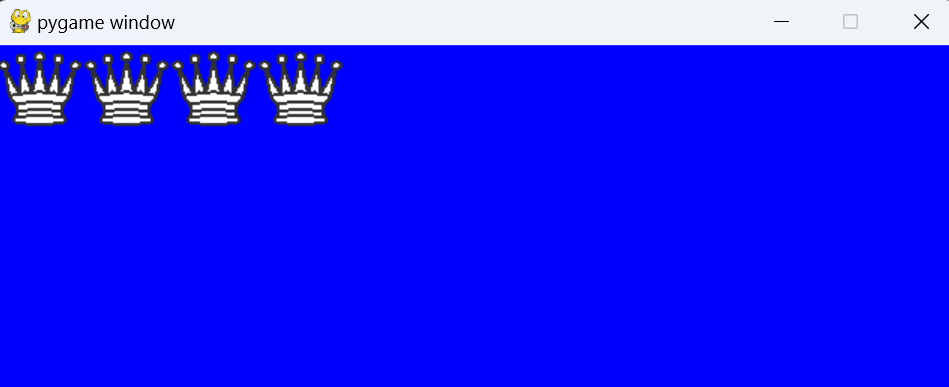
\includegraphics[width=0.9\textwidth]{imagenes/p_ej2c.png}
      \end{minipage}
    \end{itemize}

  \pagebreak

  \item \textbf{Se crea el archivo ``Ejercicio2d.py``}
  
  \vspace{\baselineskip}

  Utilizando las funciones creadas anteriormente, se contruye de acuerdo a la imagen dada en el laboratorio.

    \begin{lstlisting}[style=python]
    from interpreter import draw
    from chessPictures import *

    squares = square.join(square.negative())

    draw(squares.horizontalRepeat(4))
    \end{lstlisting}

    \vspace{\baselineskip}

    \begin{itemize}
      \item Se ejecuta de la siguiente manera.

      \begin{lstlisting}[style=shell]
      (my_env) C:\Users\melsy\Lab04\my_env\Scripts\propuestos>python Ejercicio2d.py
      pygame 2.4.0 (SDL 2.26.4, Python 3.11.1)
      Hello from the pygame community. https://www.pygame.org/contribute.html
      \end{lstlisting}

      \vspace{2\baselineskip}

      \item El resultado es:
      
      \vspace{\baselineskip}

      \begin{minipage}{\linewidth}
        \centering
        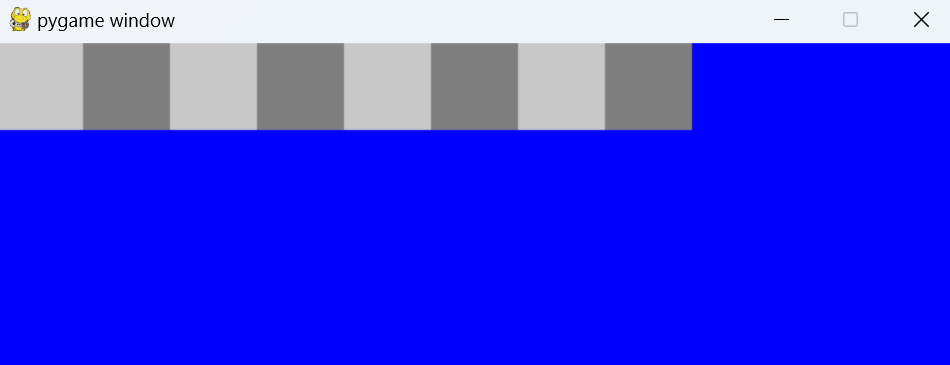
\includegraphics[width=0.9\textwidth]{imagenes/p_ej2d.png}
      \end{minipage}
    \end{itemize}

  \pagebreak

  \item \textbf{Se crea el archivo ``Ejercicio2e.py``}
  
  \vspace{\baselineskip}

  Utilizando las funciones creadas anteriormente, se contruye de acuerdo a la imagen dada en el laboratorio.

    \begin{lstlisting}[style=python]
    from interpreter import draw
    from chessPictures import *

    squares = square.negative().join(square)

    draw(squares.horizontalRepeat(4))
    \end{lstlisting}

    \vspace{\baselineskip}

    \begin{itemize}
      \item Se ejecuta de la siguiente manera.

      \begin{lstlisting}[style=shell]
      (my_env) C:\Users\melsy\Lab04\my_env\Scripts\propuestos>python Ejercicio2e.py
      pygame 2.4.0 (SDL 2.26.4, Python 3.11.1)
      Hello from the pygame community. https://www.pygame.org/contribute.html
      \end{lstlisting}

      \vspace{2\baselineskip}

      \item El resultado es:
      
      \vspace{\baselineskip}

      \begin{minipage}{\linewidth}
        \centering
        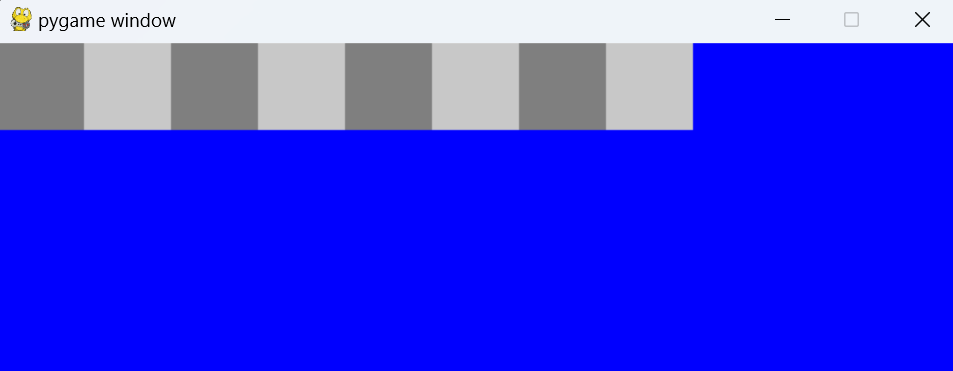
\includegraphics[width=0.9\textwidth]{imagenes/p_ej2e.png}
      \end{minipage}
    \end{itemize}

  \pagebreak

  \item \textbf{Se crea el archivo ``Ejercicio2f.py``}
  
  \vspace{\baselineskip}

  Utilizando las funciones creadas anteriormente, se contruye de acuerdo a la imagen dada en el laboratorio.

    \begin{lstlisting}[style=python]
    from interpreter import draw
    from chessPictures import *

    squares1 = square.negative().up(square)
    squares2 = square.up(square.negative())

    finalSquares = squares1.join(squares2)

    draw(finalSquares.verticalRepeat(2).horizontalRepeat(4))
    \end{lstlisting}

    \vspace{\baselineskip}

    \begin{itemize}
      \item Se ejecuta de la siguiente manera.

      \begin{lstlisting}[style=shell]
      (my_env) C:\Users\melsy\Lab04\my_env\Scripts\propuestos>python Ejercicio2f.py
      pygame 2.4.0 (SDL 2.26.4, Python 3.11.1)
      Hello from the pygame community. https://www.pygame.org/contribute.html
      \end{lstlisting}

      \vspace{2\baselineskip}

      \item El resultado es:
      
      \vspace{\baselineskip}

      \begin{minipage}{\linewidth}
        \centering
        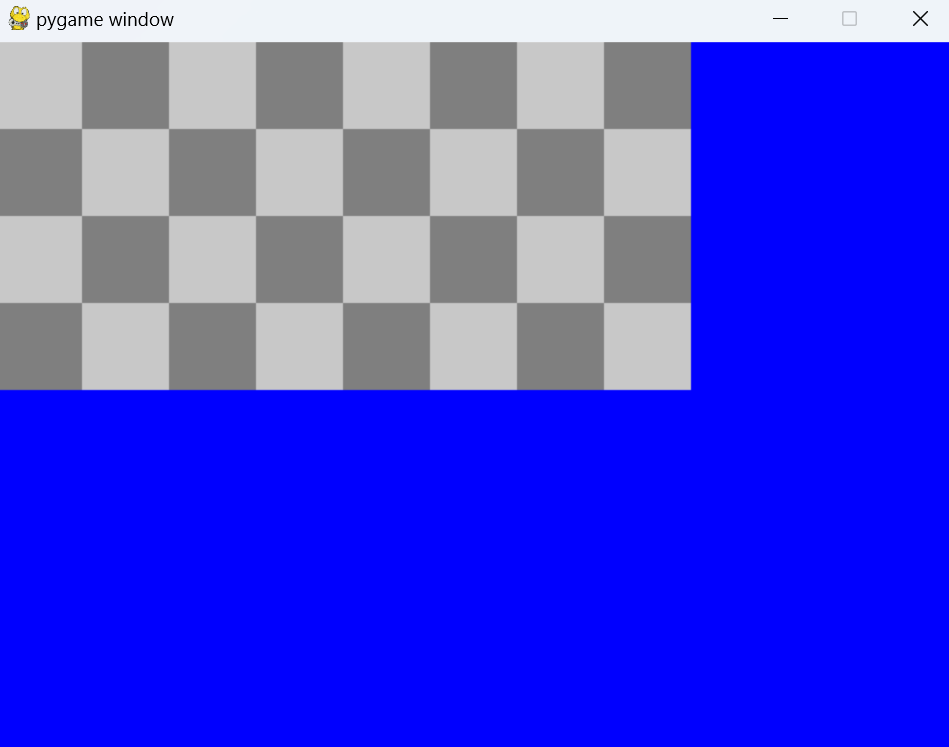
\includegraphics[width=0.9\textwidth]{imagenes/p_ej2f.png}
      \end{minipage}
    \end{itemize}

  \pagebreak

  \item \textbf{Se crea el archivo ``Ejercicio2g.py``}
  
  \vspace{\baselineskip}
  
  Utilizando las funciones creadas anteriormente, se contruye de acuerdo a la imagen dada en el laboratorio.

    \begin{lstlisting}[style=python]
    from interpreter import draw
    from chessPictures import *

    wSquare = square
    bSquare = square.negative()

    wPawns = wSquare.under(pawn).join(bSquare.under(pawn)).horizontalRepeat(4)
    bPawns = wPawns.negative()

    wPieces = bSquare.under(rock).join(wSquare.under(knight)).join(bSquare.under(bishop)).join(wSquare.under(queen)).join(bSquare.under(king)).join(wSquare.under(bishop)).join(bSquare.under(knight)).join(wSquare.under(rock))
    bPieces = wPieces.negative()

    squares1 = bSquare.up(wSquare)
    squares2 = wSquare.up(bSquare)

    finalSquares = squares1.join(squares2).verticalRepeat(2).horizontalRepeat(4)

    draw(wPieces.up(wPawns.up(finalSquares.up(bPawns.up(bPieces)))))
    \end{lstlisting}

    \vspace{\baselineskip}

    \begin{itemize}
      \item Se ejecuta de la siguiente manera.

      \begin{lstlisting}[style=shell]
      (my_env) C:\Users\melsy\Lab04\my_env\Scripts\propuestos>python Ejercicio2g.py
      pygame 2.4.0 (SDL 2.26.4, Python 3.11.1)
      Hello from the pygame community. https://www.pygame.org/contribute.html
      \end{lstlisting}

      \vspace{\baselineskip}

      \item El resultado es:
      
      \vspace{\baselineskip}

      \begin{minipage}{\linewidth}
        \centering
        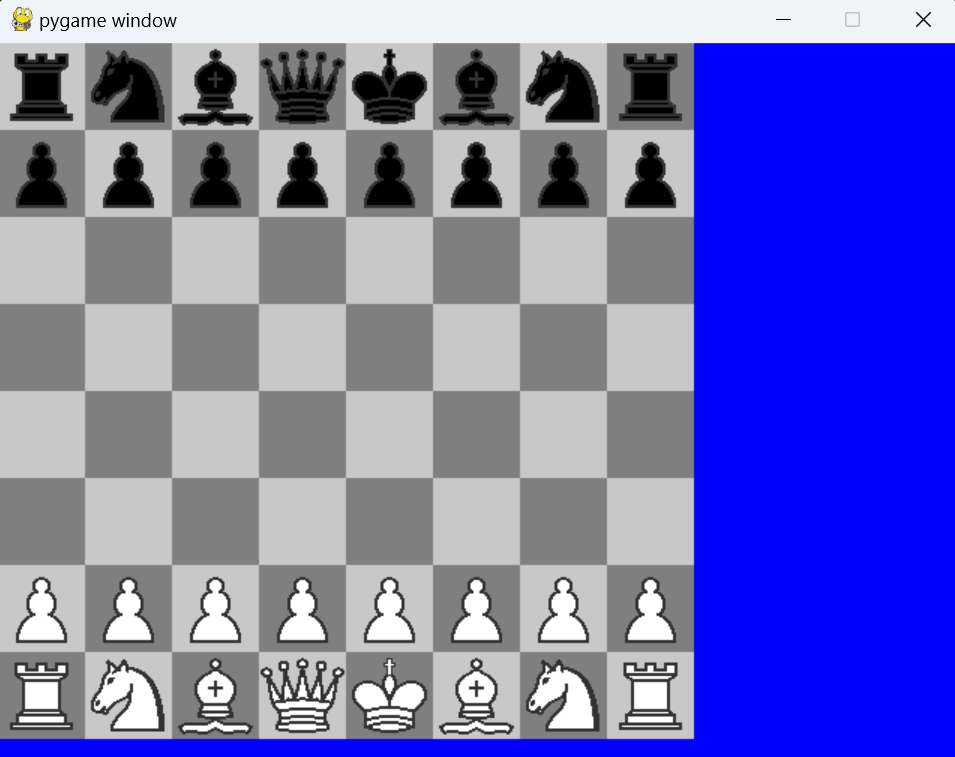
\includegraphics[width=0.6\textwidth]{imagenes/p_ej2g.png}
      \end{minipage}
    \end{itemize}

  \pagebreak

  \item \textbf{Se crea el archivo ``PruebaRotate.py``}
  
  \vspace{\baselineskip}
  
  Este es una figura extra que se creo en base a ``Ejercicio2g.py``, pero que se muestra el tablero de manera que ha rotado 90 grados.

    \begin{lstlisting}[style=python]
    from interpreter import draw
    from chessPictures import *

    wSquare = square
    bSquare = square.negative()

    wPawns = wSquare.under(pawn).join(bSquare.under(pawn)).horizontalRepeat(4)
    bPawns = wPawns.negative()

    wPieces = bSquare.under(rock).join(wSquare.under(knight)).join(bSquare.under(bishop)).join(wSquare.under(queen)).join(bSquare.under(king)).join(wSquare.under(bishop)).join(bSquare.under(knight)).join(wSquare.under(rock))
    bPieces = wPieces.negative()

    squares1 = bSquare.up(wSquare)
    squares2 = wSquare.up(bSquare)

    finalSquares = squares1.join(squares2).verticalRepeat(2).horizontalRepeat(4)

    tabla = wPieces.up(wPawns.up(finalSquares.up(bPawns.up(bPieces))))

    draw(tabla.rotate())
    \end{lstlisting}

    \vspace{\baselineskip}

    \begin{itemize}
      \item Se ejecuta de la siguiente manera.

      \begin{lstlisting}[style=shell]
      (my_env) C:\Users\melsy\Lab04\my_env\Scripts\propuestos>python PruebaRotate.py
      pygame 2.4.0 (SDL 2.26.4, Python 3.11.1)
      Hello from the pygame community. https://www.pygame.org/contribute.html
      \end{lstlisting}

      \vspace{\baselineskip}

      \item El resultado es:
      
      \vspace{\baselineskip}

      \begin{minipage}{\linewidth}
        \centering
        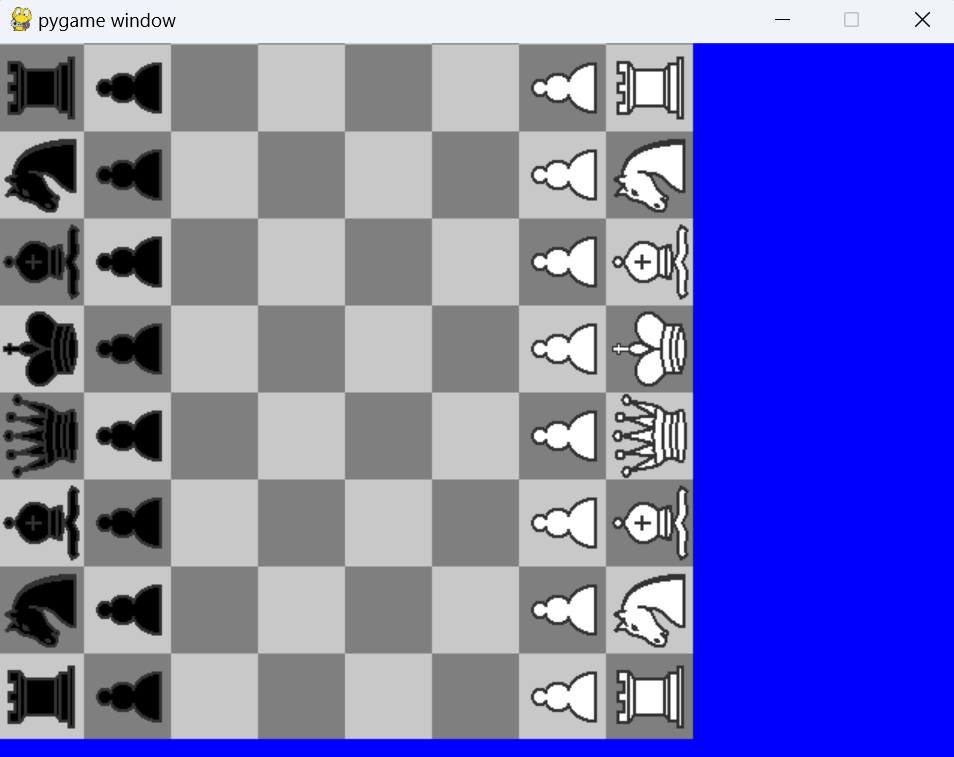
\includegraphics[width=0.6\textwidth]{imagenes/p_ej2extra.png}
      \end{minipage}
    \end{itemize}

  \end{itemize}

\pagebreak

\subsection*{COMMITS MÁS IMPORTANTES}

\vspace{\baselineskip}

\begin{minipage}{\linewidth}
  \centering
  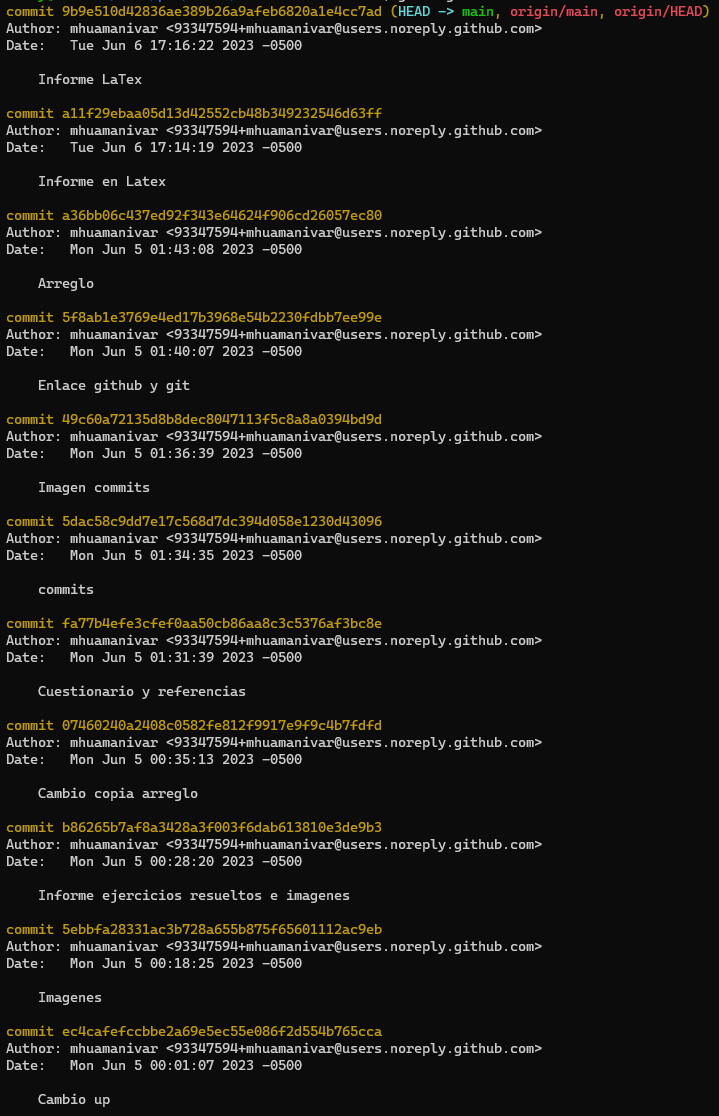
\includegraphics[width=0.85\textwidth]{imagenes/commits1.png}
\end{minipage}

\pagebreak

\begin{minipage}{\linewidth}
  \centering
  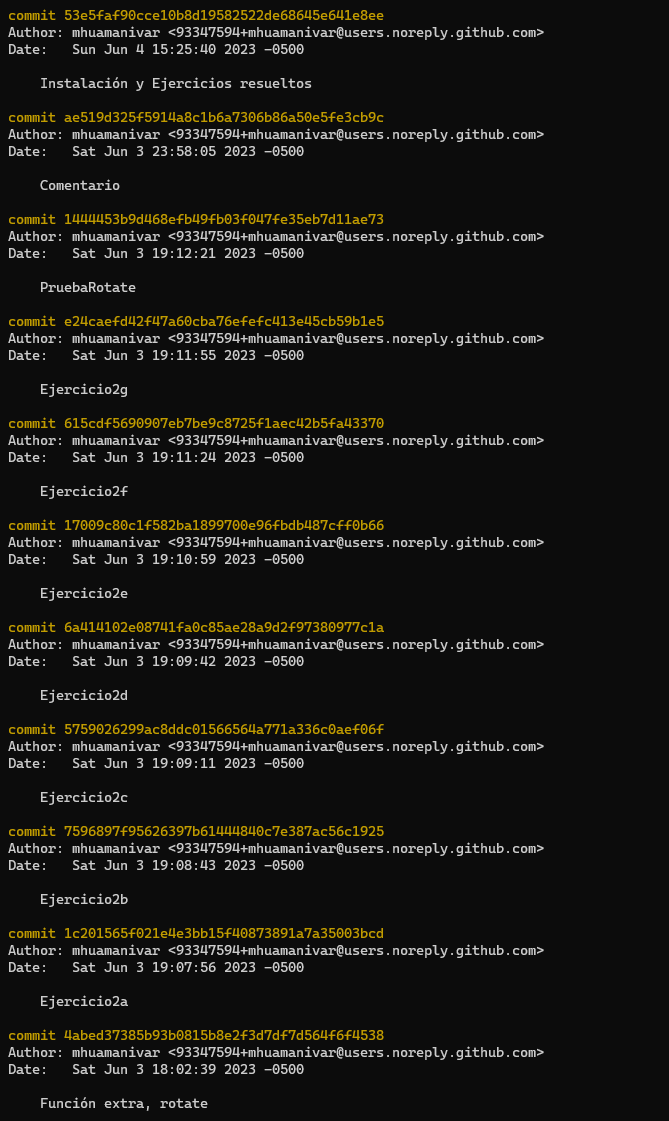
\includegraphics[width=0.85\textwidth]{imagenes/commits2.png}
\end{minipage}

\pagebreak

\begin{minipage}{\linewidth}
  \centering
  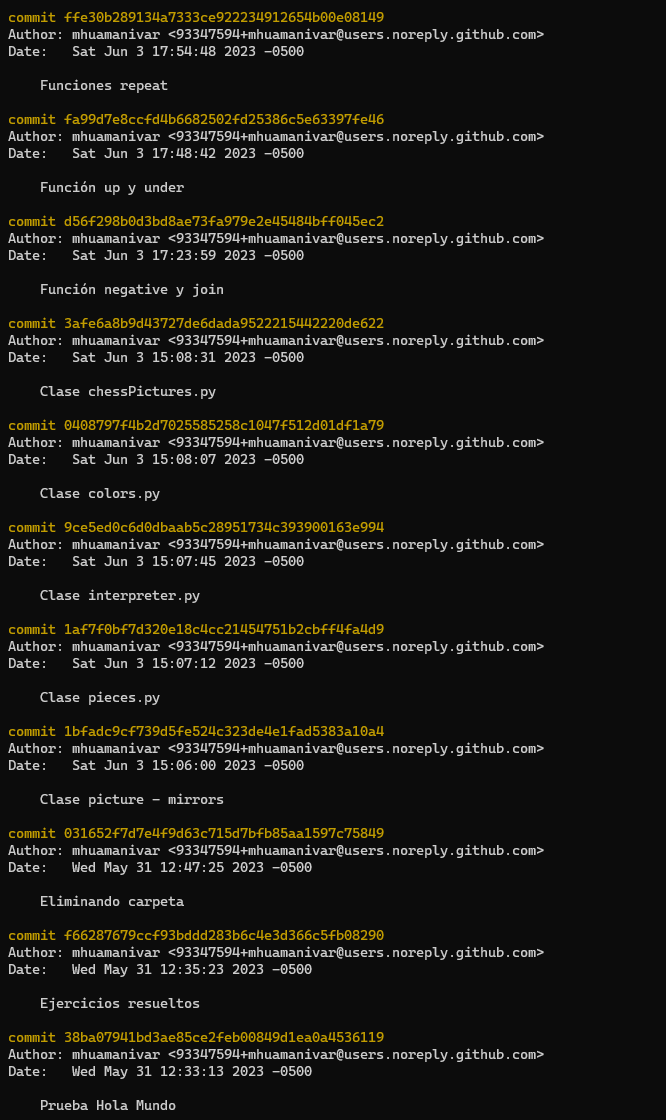
\includegraphics[width=0.85\textwidth]{imagenes/commits3.png}
\end{minipage}

\pagebreak


\noindent
\section*{\centering CUESTIONARIO}

\vspace{2\baselineskip}

\begin{itemize}
  \item \textbf{¿Qué son los archivos ``.pyc``?}
  
  Son los archivos compilados de Python, es una versión de un módulo que ya ha sido compilado en bytes con éxito. Sin embargo, si la compilación falla, entonces el archivo ``.pyc`` sera reconocido como inválido. En los archivos ``.pyc`` se deben tener en cuenta ciertas características:
  
  \begin{itemize}
    \item Cuando el intérprete de Python es invocado con flag ``-o``, entonces los archivos que son compilados son optimizados y eliminan datos no importantes, por lo que ya no son ``.pyc``, sino que son ``.pyo``.
    \item El programa no compila más rápido si es que ejecutar los ``.pyc``, lo único en lo que son rápidos es la velocidad con la que se cargan.
    \item Es posible que existan archivos ``.pyc``, sin la necesidad de haber modulos con el nombre que tiene el ``.pyc``, esto puede usarse para distribuir una librería de Python.
    \item El módulo ``compile all`` puede crear archivos ``.pyc`` para todos los módulos de un directorio.
    \item Python verifica la fecha de modificación del código con la versión compilada para ver si está desactualizada y necesita ser recompilado, ya que en los archivos ``.pyc`` se puede visualizar la versión con la que ha sido compilado el módulo.
  \end{itemize}

  \vspace{\baselineskip}

  \item \textbf{¿Para qué sirve el directorio pycache?}
  
  El directorio ``\_\_pycache\_\_`` sirve para acelerar la carga de módulos, puesto que Python almacena en caché la versión compilada de cada módulo bajo el nombre de ``nombre\_de\_modulo.version.pyc``, donde se muestra la versión del formato con el que se ha compilado el archivo, el cual generalmente es el número de versíon de Python. No se recomienda borrar a menudo estos archivos ni suprimir la creación de estos ya que como han sido compilados, se estaría restando a su función principal que es acelerar el proceso de la carga de módulos.

  \vspace{\baselineskip}

  \item \textbf{¿Cuáles son los usos y lo que representa el subguión en Python?}
  
  El subguión tiene una gran variedad de usos en Python, además de una representación cuando se habla de atributos o métodos de una clase. Entre ellos tenemos:

  \begin{itemize}
    \item Para omitir valores: Es decir, podemos usarlo como una variable ``\_`` la cual solo la utilizaremos una vez, por ejemplo, en las iteraciones del ``for``. Por otro lado, cuando tenemos muchos valores y queremos seleccionar solo unos cuantos e ignorar un rango de ellos, entonces podemos utilizar ``*\_``.
    \item Como placeholder: Esto quiere decir que cuando nos encontremos en el intérprete de Python podemos guardar la anterior respuesta para utilizarla en una siguiente operación.
    \item Como namespace: Cuando queremos utilizar un nombre para una variable, pero esta ya es una palabra reservada para Python, entonces podemos utilzar ``\_`` al final del nombre de la palabra.
    \item Para números: Podemos utilizar ``\_`` para expresar números muy grandes, y queremos separar cada tres cifrar para un mejor entendimiento.
    \item Representación en clases: Cuando utilizamos ``\_`` dos veces antes y después del nombre de un atributo, de manera ``\_\_nombre\_de\_atributo\_\_``, entonces esto representa un atributo privado de la clase. Por otro lado, para los métodos, al utilizar de la siguiente manera ``\_\_nombre\_del\_metodo\_\_`` quiere decir que estos son métodos que se pueden sobreescribir facilmente en las clases que heredan, siendo esta usada en la clase padre.
  \end{itemize}

\end{itemize}

\noindent
\section*{\centering REFERENCIAS}

\vspace{2\baselineskip}

\begin{itemize}
  \item \url{https://www.w3schools.com/python/python_reference.asp}
  \item \url{https://docs.python.org/3/tutorial/}
  \item \url{https://docs.python.org/release/1.5.1p1/tut/node43.html}
  \item \url{https://docs.python.org/3/tutorial/modules.html}
  \item \url{https://pywombat.com/articles/guion-bajo-python}
\end{itemize}

\end{document}